\vspace{-0.1cm}

Naive Bayes (henceforth NB) and Logistic Regression (henceforth LogReg) classifiers are among the most popular first choices for large scale text classification problems in the industry.
We use the Naive Bayes classifier over multinomial distribution with Dirichlet prior of $1.0$ as a baseline.
This baseline has also been the choice baseline in \cite{Shen12, Sun14} for categorizing product titles at scale due to its low runtime requirements.
Naive Bayes classifier is a specialization of Logistic Regression classifier \cite{Ng01}, where the latter is much more insensitive to dataset imbalance due to optimization of log-odds ratios in the objective function and much more so in the presence of effective regularizers such as L1 and Elastic Net \cite{ESL03, Zhang04:SGD, Zou05:EN}.
We refrain from using a KNN classifier due to our very high dimensional feature spaces which can lead to prohibitively long prediction times under arbitrary feature transforms even under an efficient KD-Tree data structure \cite{Manning08:IR}.

\vspace{-0.2cm}
\subsection{Data Preprocessing}
\label{Subsect:Data-preprocessing}
\vspace{-0.2cm}

Our data preprocessing steps are minimal.
For each listing, our primary text data is the product title. 
For AmazonJ and BU2 datasets, we also extract the list price whenever available. 
Additionally for BU2 dataset, we add the leaf node of navigational breadcrumbs, whenever available, as another meta feature.
BU1 dataset only has titles.
From every such listing, we remove standard English stopwords and tokens that appear in 10 listings or less i.e. rare tokens. 
We have found out that this removal reduces vocabulary sizes by almost 50\% without reducing classification performance.
We however, do not remove stopwords for the CNN classifier.
Instead to reduce vocabulary size for CNN, we replace rare tokens by the nominal token ``[RARE]'' and all numbers by the nominal form ``[NUM]''.
Further, all text is lowercased.

\vspace{-0.1cm}
\subsection{Initial Experiments with Business Unit 1 dataset}
\label{Subsect:BU1-exp}

\begin{wrapfigure}{l}{0.71\textwidth}
	\vspace{-0.8cm}
	\centering
	\subfloat[{Prediction on 10\% test set using word unigram count features}]{\label{Figure_BU1-WUC}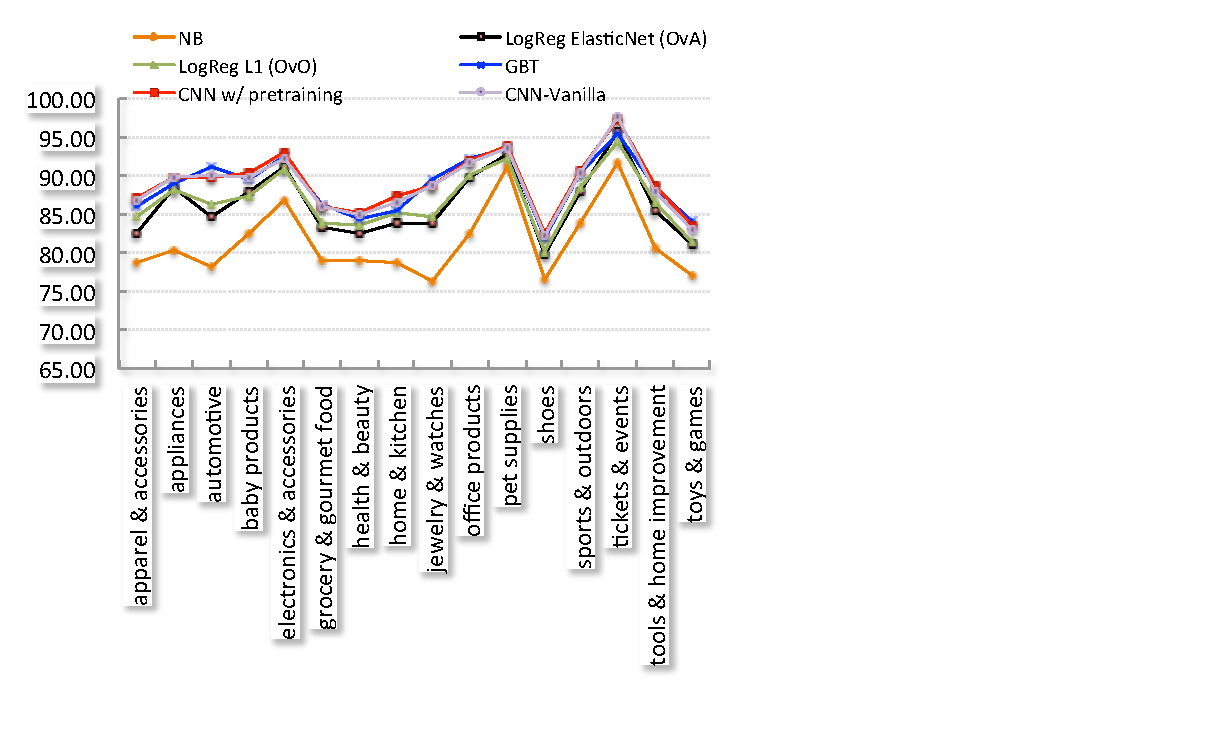
\includegraphics[width=0.35\textwidth]{images/BU1-WUC-predictions}} \hspace{0.05cm}
	\subfloat[{Prediction on 10\% test set using word unigram bi-positional count features}]{\label{Figure_BU1-WUBPC}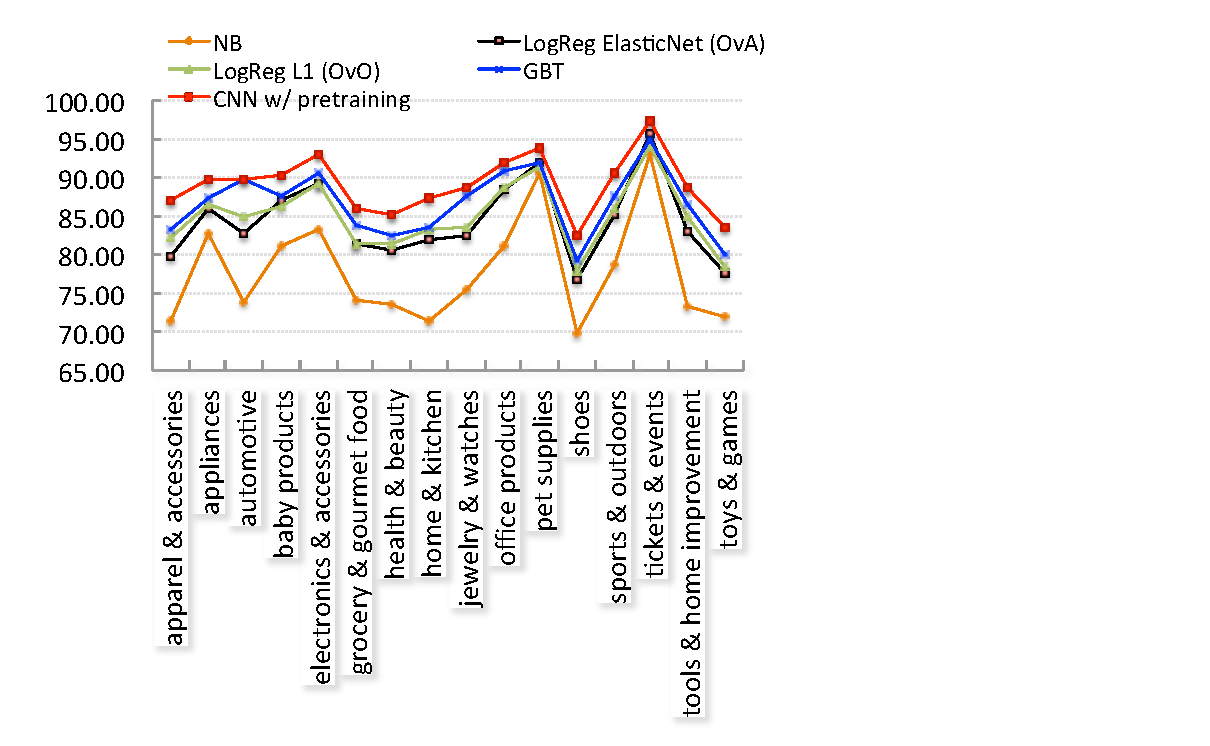
\includegraphics[width=0.35\textwidth]{images/BU1-WUBPC-predictions}} 

	\subfloat[{Prediction on 10\% test set using word bigram count features}]{\label{Figure_BU1-WBC}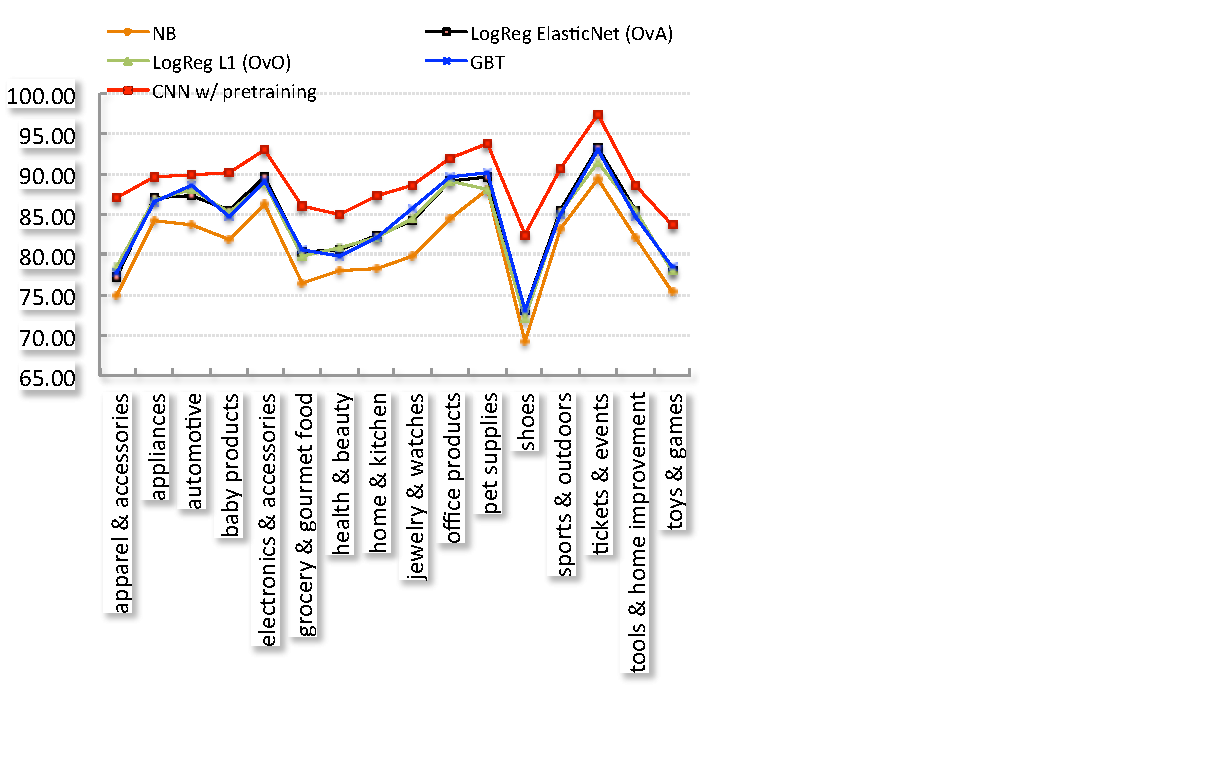
\includegraphics[width=0.35\textwidth]{images/BU1-WBC-predictions}} \hspace{0.05cm}
	\subfloat[{Prediction on 10\% test set using word bigram bi-positional count features}]{\label{Figure_BU1-WBBPC}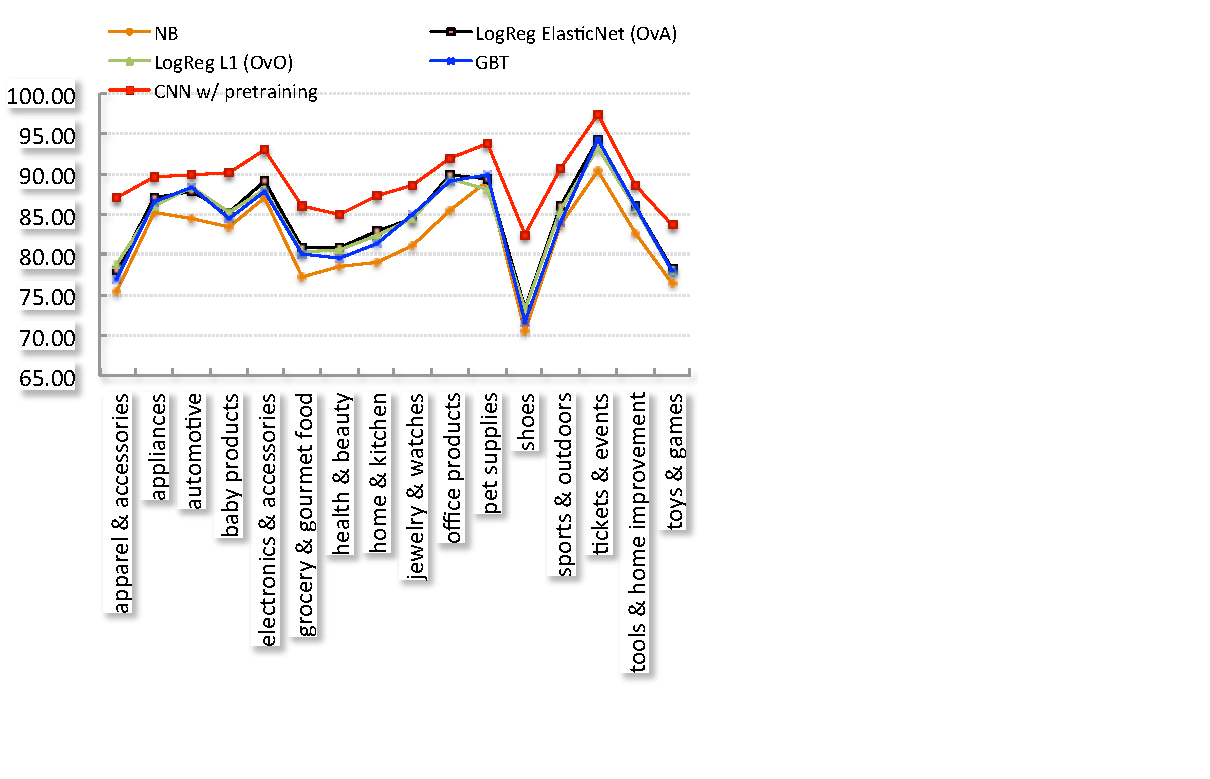
\includegraphics[width=0.35\textwidth]{images/BU1-WBBPC-predictions}} 
	\caption{\small{Predictions on BU1 test set for different classifiers. The CNN classifier has only one configuration and thus shows constant curves in all plots. Best viewed in color.} }
	\label{Figure_BU1-predictions}
	\vspace{-0.3cm}
\end{wrapfigure}
Our initial experiments with NB also consisted of using three other features -- a word bigram feature, a bi-positional word unigram feature and a bi-positional word bigram feature.
Consider a title text ``\textit{120gb hd 5400rpm sata fdb 2 5 mobile}'' from the ``\textbf{Data storage}'' leag node of Electronics taxonomy subtree and another title text ``\textit{acer aspire v7 582pg 6421 touchscreen ultrabook 15 6 full hd intel i5 4200u 8gb ram 1tb hdd 20gb ssd nvidia geforce gt 720m}'' from the ``\textbf{Laptops and netbooks}'' leaf node of the same subtree.
For bi-positional features, we split the length of the title in half and augment word uni/bi-grams with a left/right-half position. It was observed that some merchants would put laptop specific words up front and storage and peripheral specific words later for the listings in ``Laptops'' leaf node while the opposite for listings in ``Data storage'' leaf node.
This educated guess did help NB significantly (Fig. \ref{Figure_BU1-predictions-feature-averages}) but not the other classifiers.
For feature values, we use the feature descriptor counts within the title, except that of list price whose value we use directly (with rounding in NB classifier).
In the legends in all figures henceforth, ``OvO'' means ``One vs. One'' and ``OvA'' means ``One vs All''; L1 means L1 regularization \cite{LibLinear} and ElasticNet \cite{Zou05:EN} is a linear combination of 15\% L1 regularization and 85\% L2 regularization.
\begin{wrapfigure}{r}{0.45\textwidth}
	\vspace{-0.6cm}
	\centering
	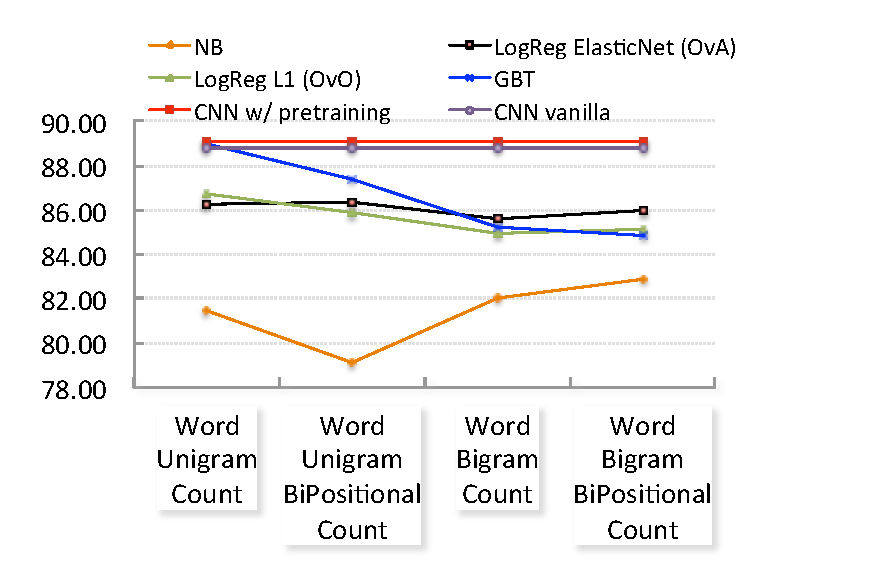
\includegraphics[width=0.43\textwidth]{images/BU1-mean-micro-precision}
	\caption{\small{Mean micro precisions of different classifiers over different feature setups except CNN.}}
	\label{Figure_BU1-predictions-feature-averages}
	\vspace{-0.4cm}
\end{wrapfigure}
For CNN experiments, we use an adaptation of TensorFlow \cite{TensorFlow}.

We observe from Figs. \ref{Figure_BU1-WUC}, \ref{Figure_BU1-WUBPC}, \ref{Figure_BU1-WBC} and \ref{Figure_BU1-WBBPC} that word unigram count features perform very well except NB and we decide to use this feature in all of our subsequent experiments.
Additionally, the micro precisions (and F1s) of CNN and GBT are statistically significant than the other classifiers for BU1 dataset over word unigrams under a paired t-test with a p-value $<$ at least $0.0001$. 
%% TODO: Pew Putthividya POS ??




\subsection{Classification Improvements with List Price on BU2 Dataset}
\label{Subsect:BU2-classification-improve-list-price}

Hello world
\begin{wrapfigure}{l}{0.5\textwidth}
	\centering
	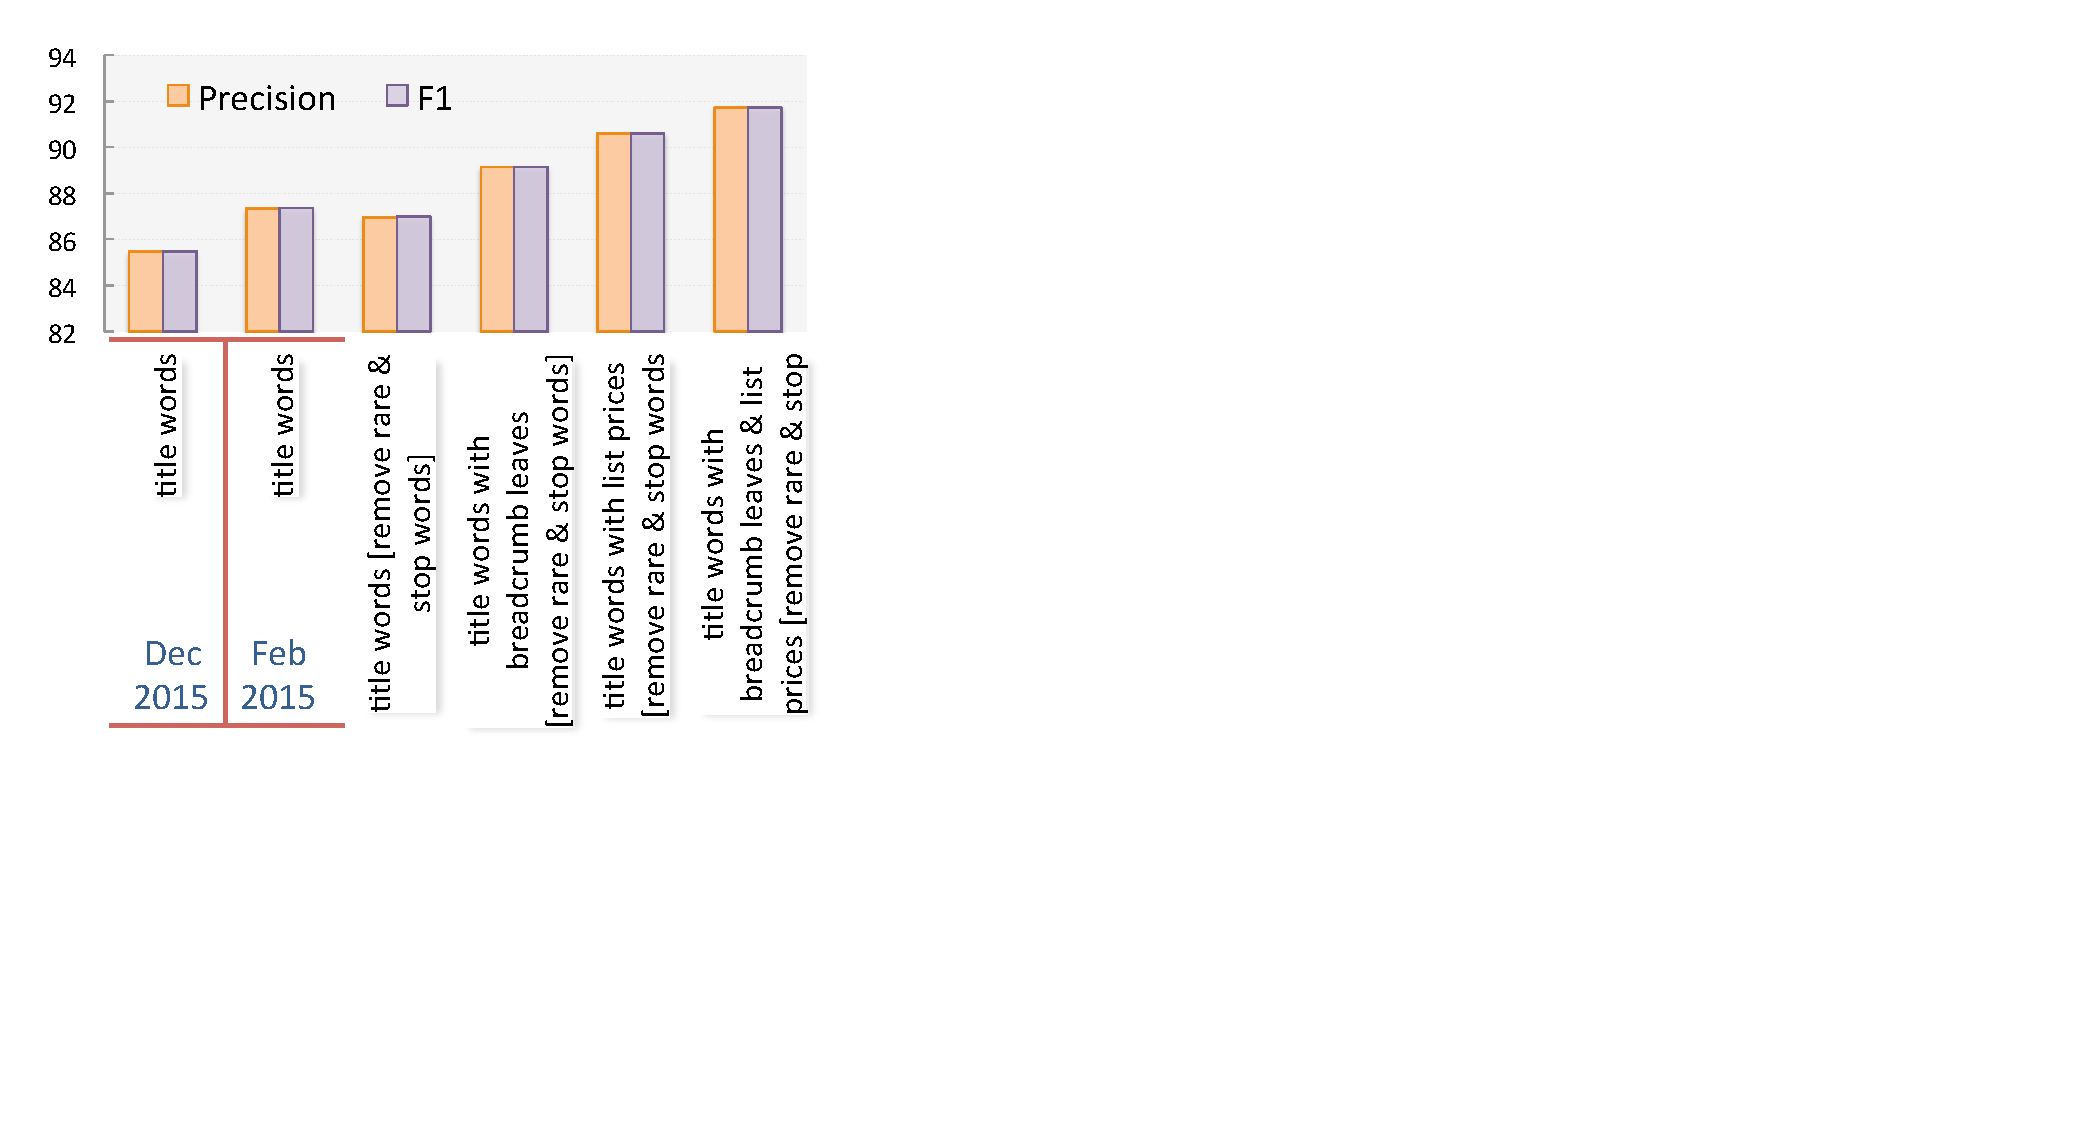
\includegraphics[width=0.48\textwidth]{images/BU2-gbt-feature-improvements}
	\caption{Improvements in classification performance of GBTs over different feature sets on the Women's Clothing category of BU2 dataset}
	\label{Figure_BU2-gbt-feature-improvements}
\end{wrapfigure}
Some text

\subsection{Noise Analysis of Business Unit 2 Dataset using Correspondence LDA}
\label{Subsect:BU2-noise-analysis}

\begin{wrapfigure}{l}{0.4\textwidth}
	\vspace{-0.8cm}
	\centering
	\subfloat[{Latent ``noise'' topics over listings in \textbf{Shoes} taxonomy subtree. }]{\label{Figure_BU2-noise-topics}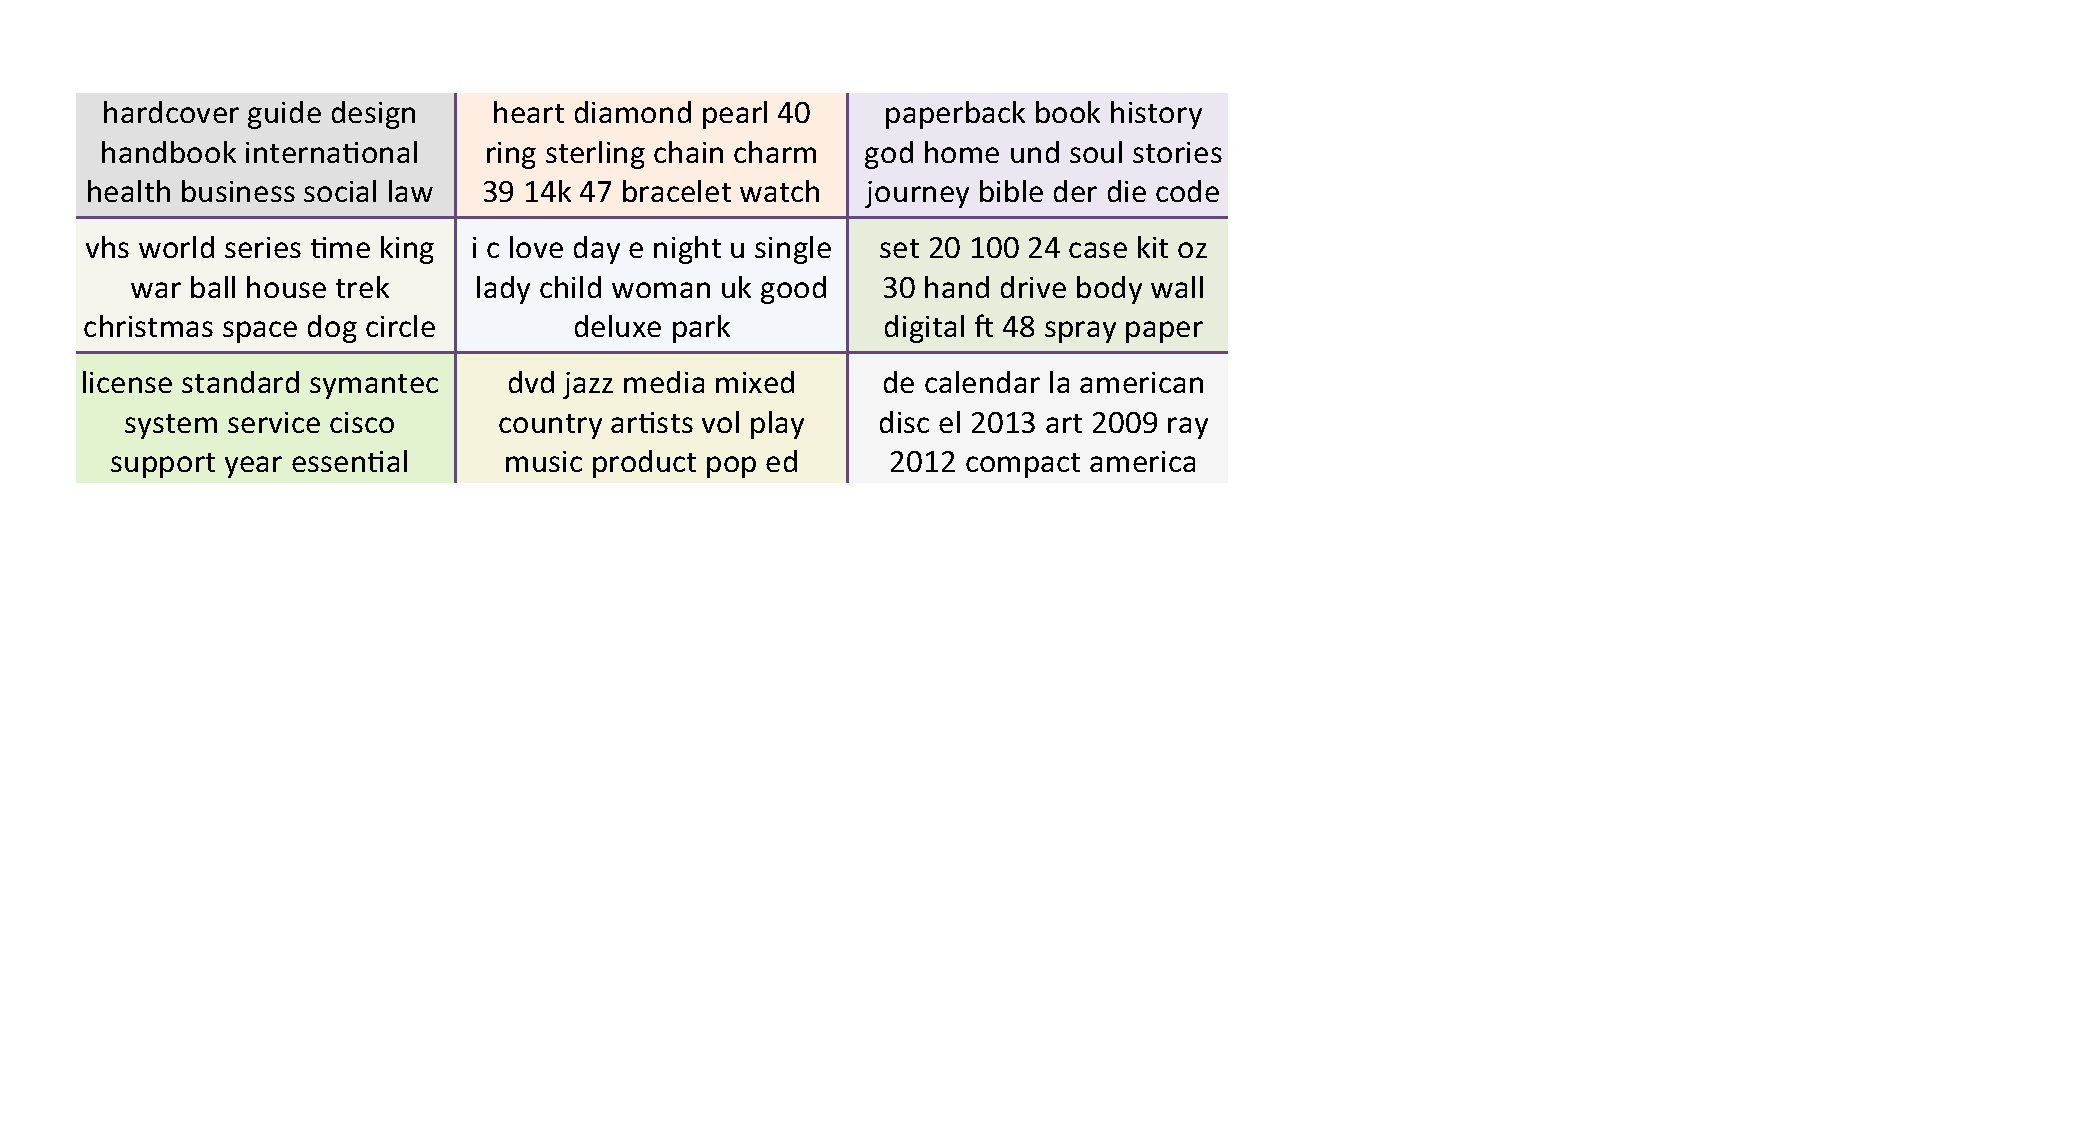
\includegraphics[width=0.4\textwidth]{images/BU2-noise-topics}}
	\vspace{-0.3cm}
\end{wrapfigure}	
	
\begin{wrapfigure}{r}{0.6\textwidth}
	\vspace{-0.8cm}
	\centering
	\subfloat[{Interpretation of latent topics using a GBT model trained on noisy Feb 2016 snapshot of BU2 dataset. data}]{\label{Figure_BU2-topic-annotation}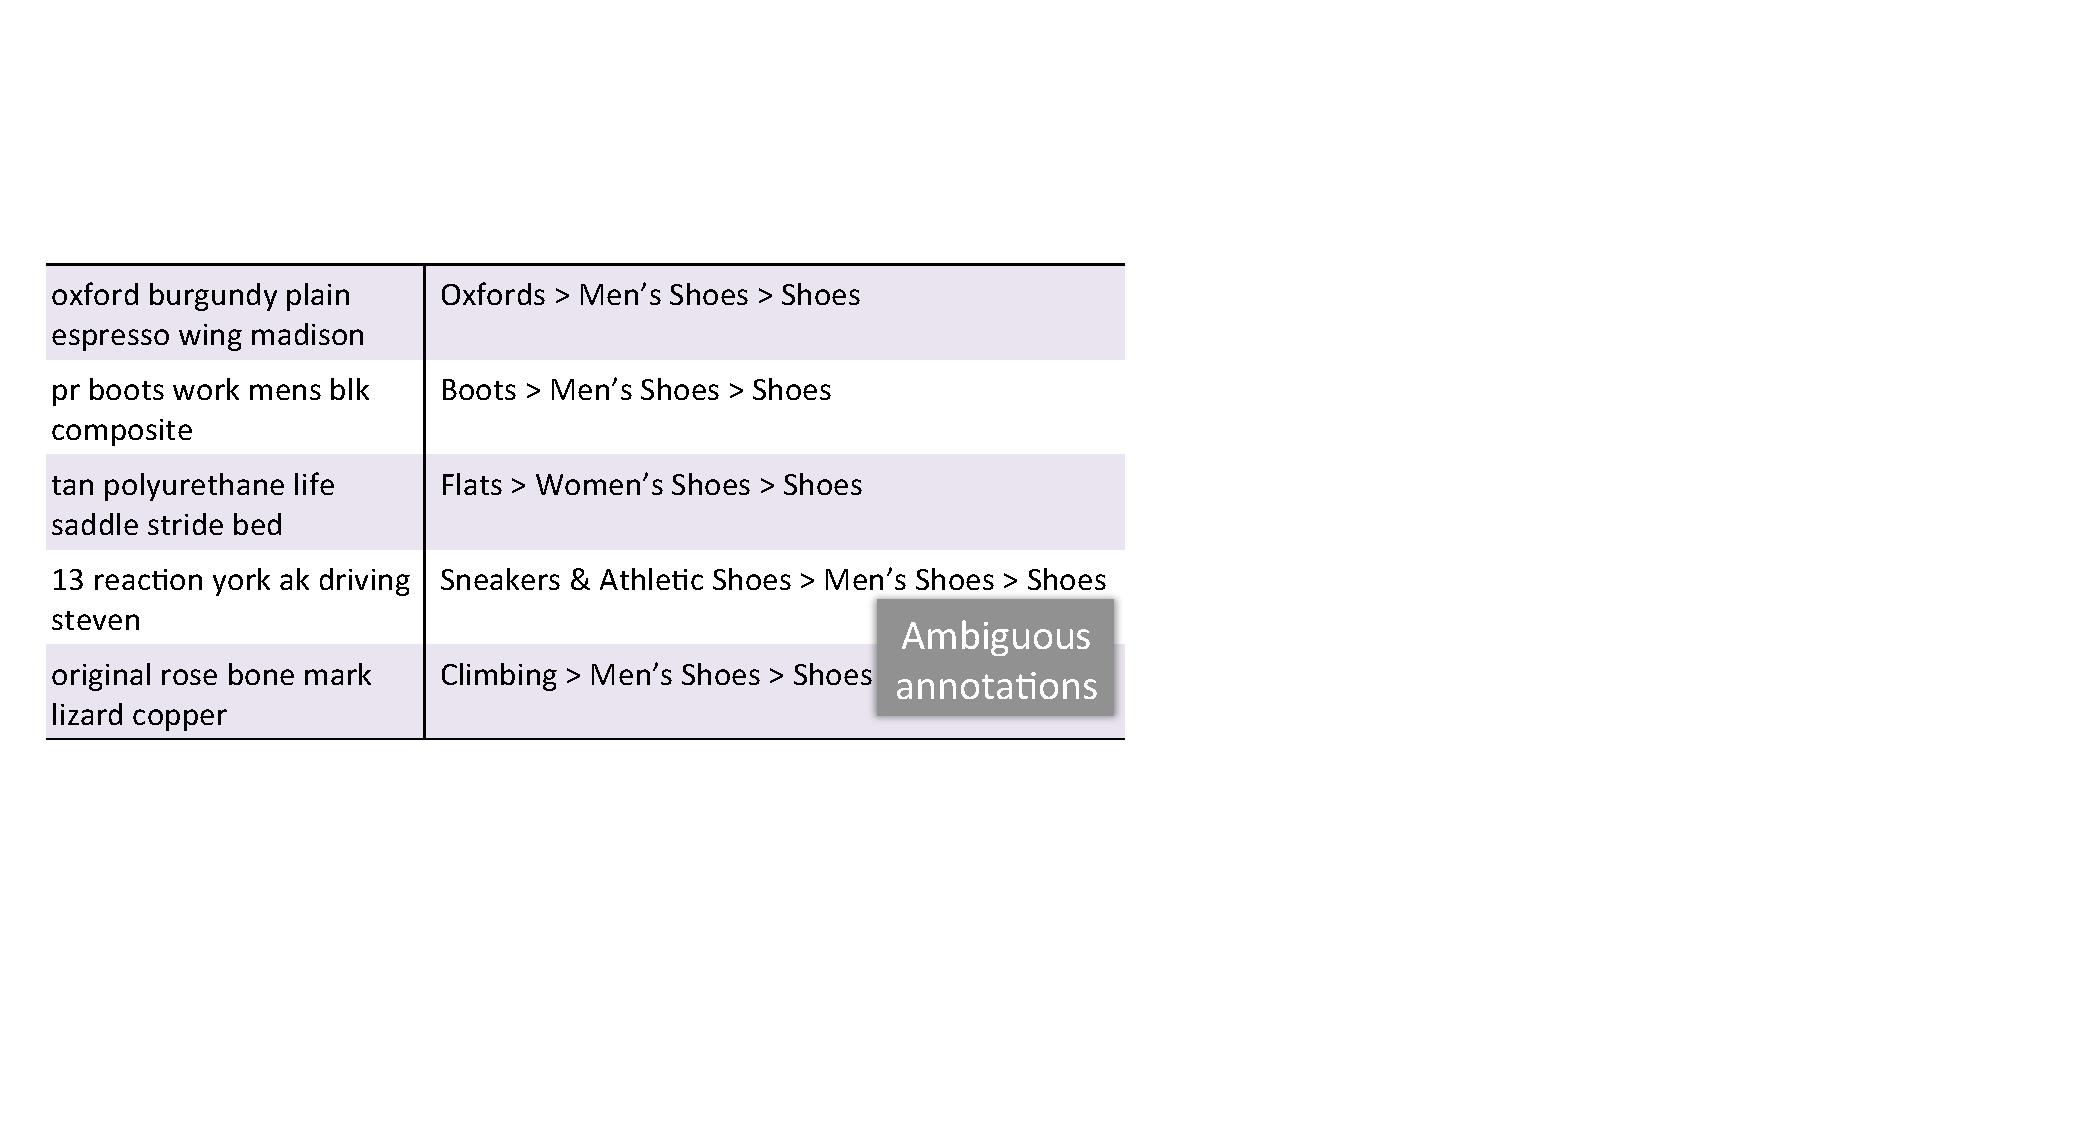
\includegraphics[width=0.6\textwidth]{images/BU2-topic-annotation}}
	\vspace{-0.3cm}
\end{wrapfigure}
Hello noise


